\chapter{Results}

In this chapter we present the results of semi-supervised learning of jointly aligned embeddings, where ``jointly aligned" means that embeddings for both domains and the mapping from one to the other are all learned simultaneously. 


\section{Summary}
\begin{itemize}
    \item Alignment accuracies of greater than 95\% were achieved for both domains ($f(x) \rightarrow y$ and $g(y) \rightarrow x$).
    \item Visualisation of the jointly aligned embeddings through t-SNE dimensionality reduction showed good clustering behaviour with semantically meaningful clusters.
    \item Aligned embeddings were found to be of higher quality compared to independently learned embeddings, when using a similarity metric based on the WordNet lexical database. Specific definitions of ``quality" and ``similarity" are given in a later section.
    \item Aligned embeddings were found to be less stable compared to independently learned embeddings. 
    \item The MMD metric increased alignment accuracy, but sometimes decreased embedding quality. 
\end{itemize}


\section{Visualising clusters}
Similar to what was done with the independently learned embeddings, we run the t-SNE algorithm on the aligned embeddings for both domains, and plot the results.

In Figures \ref{fig:openimagesaligned} and \ref{fig:audiosetaligned} below, the blue points represent the concepts in the intersection i.e. they are present in both Open Images and AudioSet. The orange points represent the concepts that are in the 300 most frequent for the respective domain that are not also in the intersection. Only the t-SNE plots for alignment run without MMD are shown, as the plots for alignment run with MMD look materially similar. 

\begin{figure}[H]
    \centering
    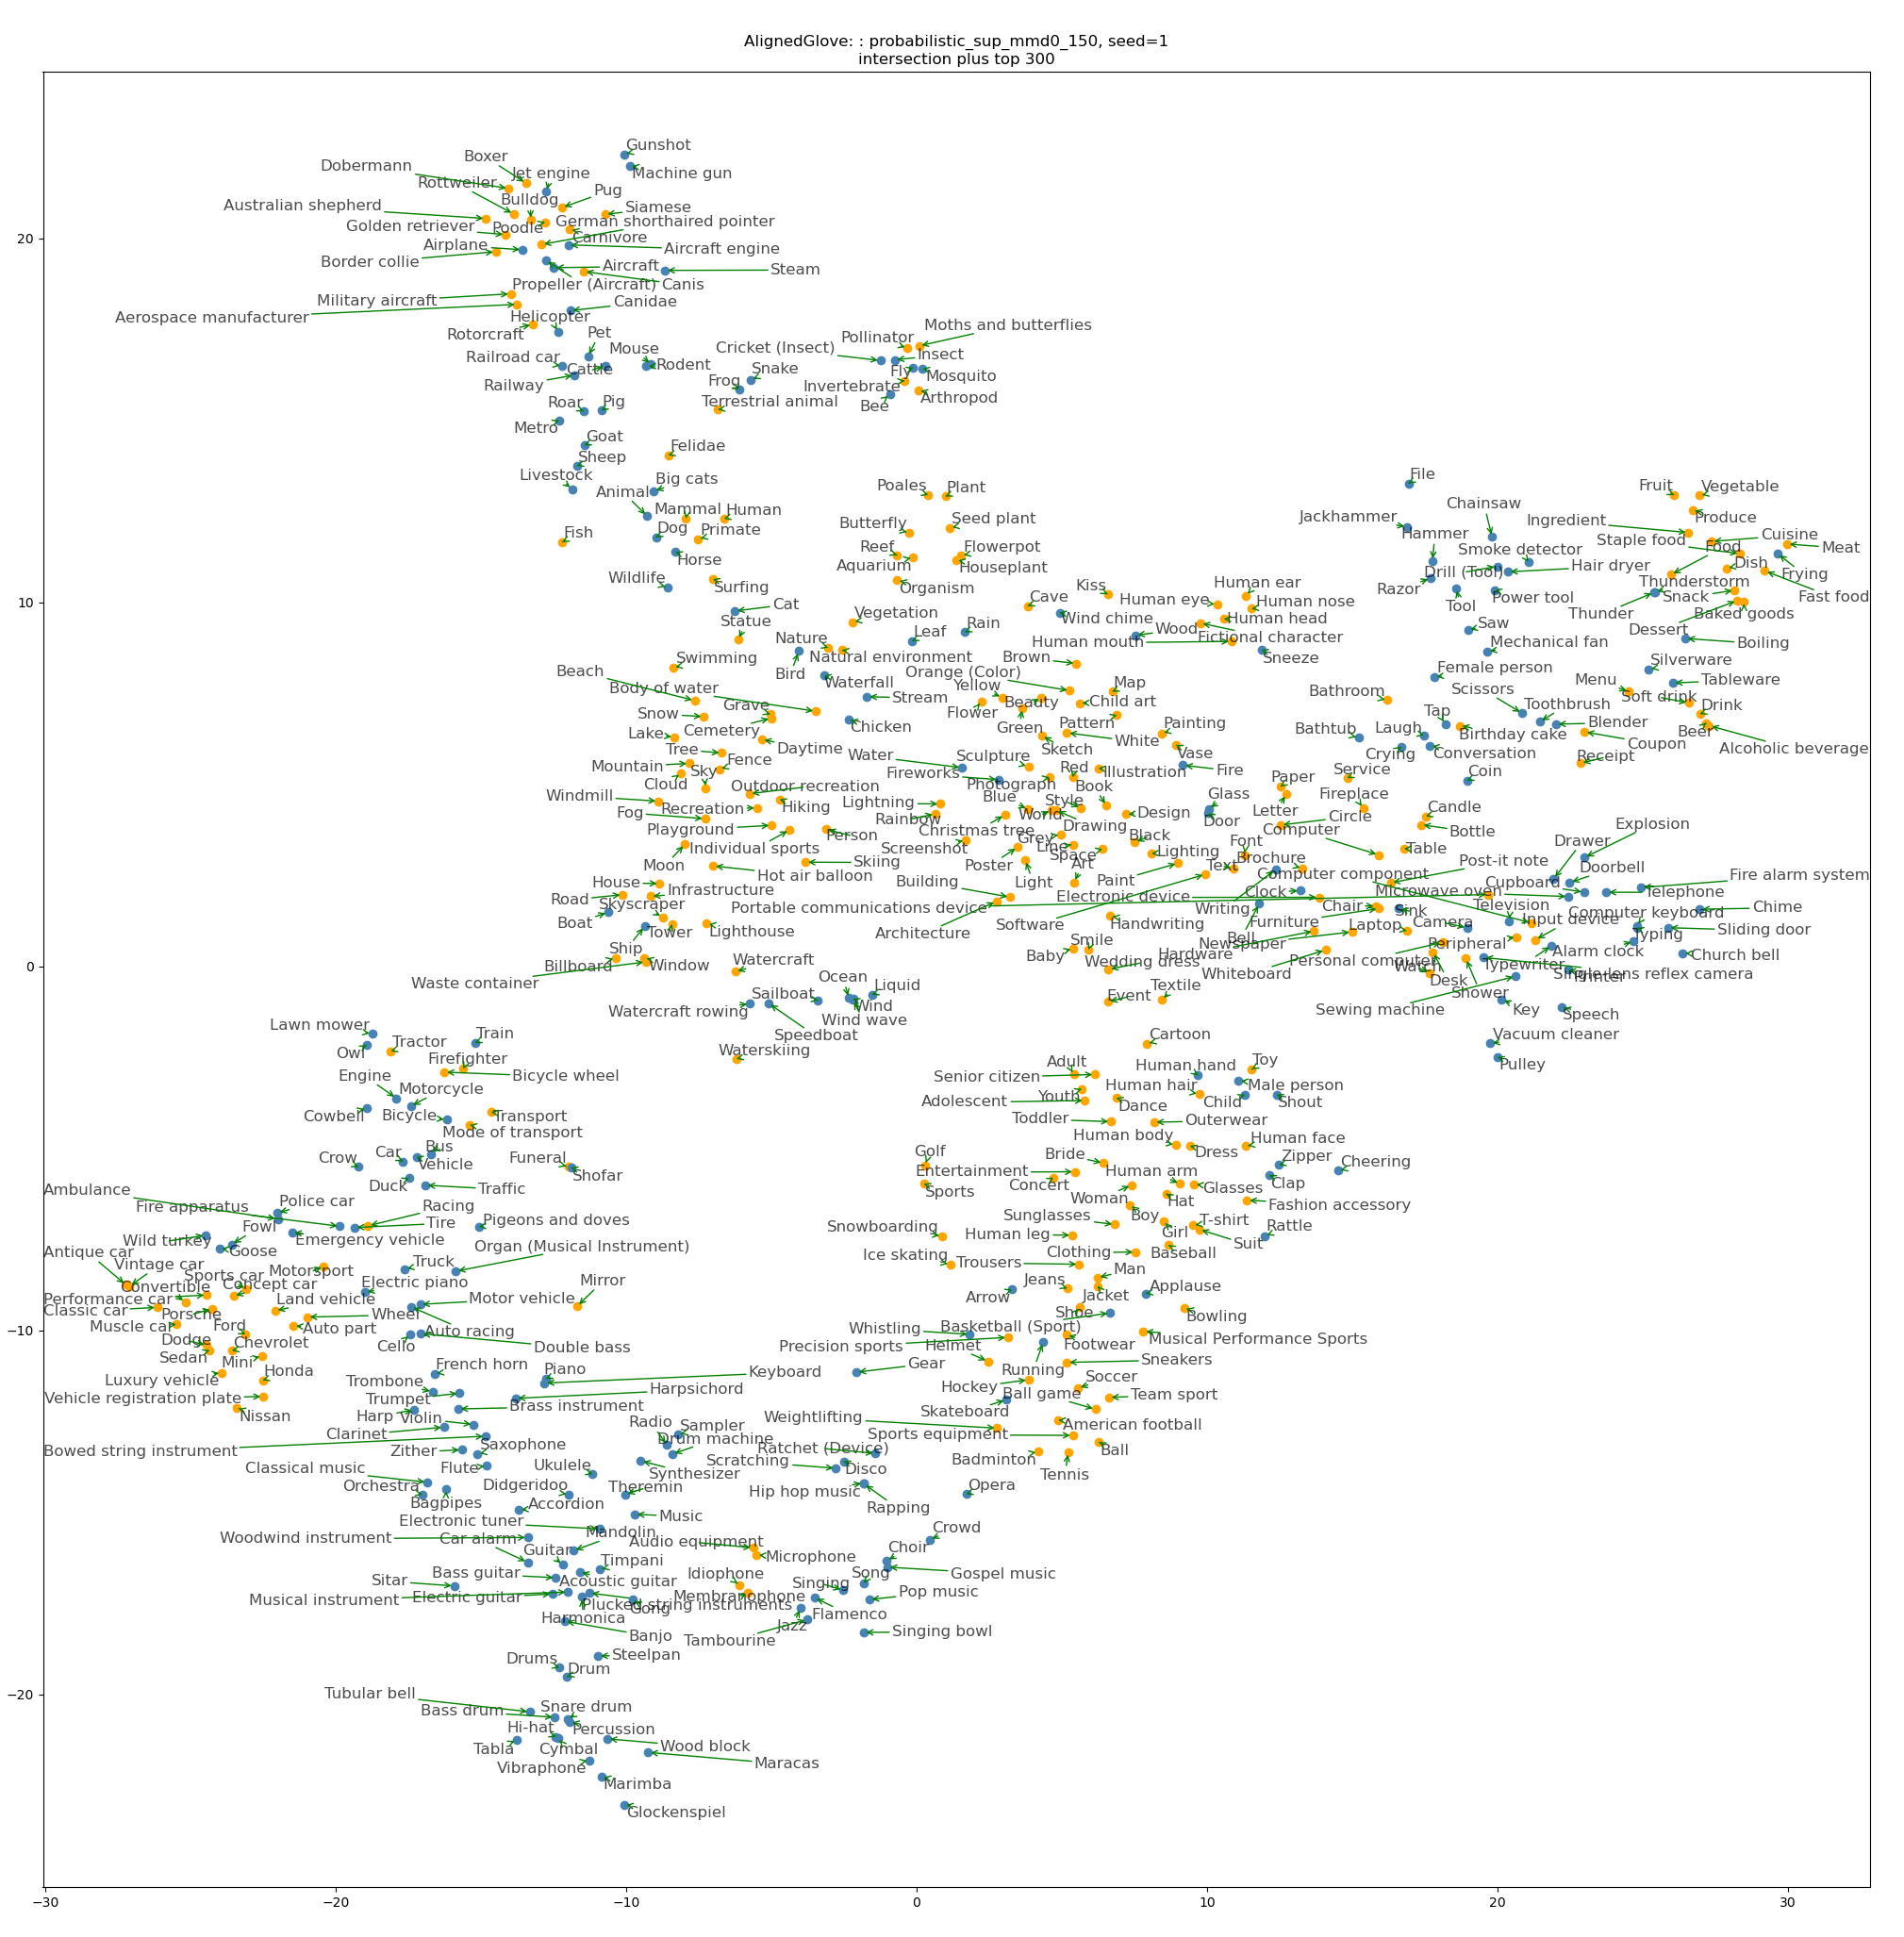
\includegraphics[width=\textwidth]{images/results/intersection_top300_tsne_openimages_probabilistic_sup_mmd0_150_AlignedGlove_1.png}
    \caption{
        \label{fig:openimagesaligned}
        t-SNE plot of concept embeddings for Open Images that are in the intersection of both domains (blue points) or in the top 300 most frequent (orange points). These are the embeddings for alignment run without MMD. See Figure \ref{fig:openimageszoom} for zoomed-in examples. 
    }
\end{figure}

\begin{figure}[H]
    \centering
    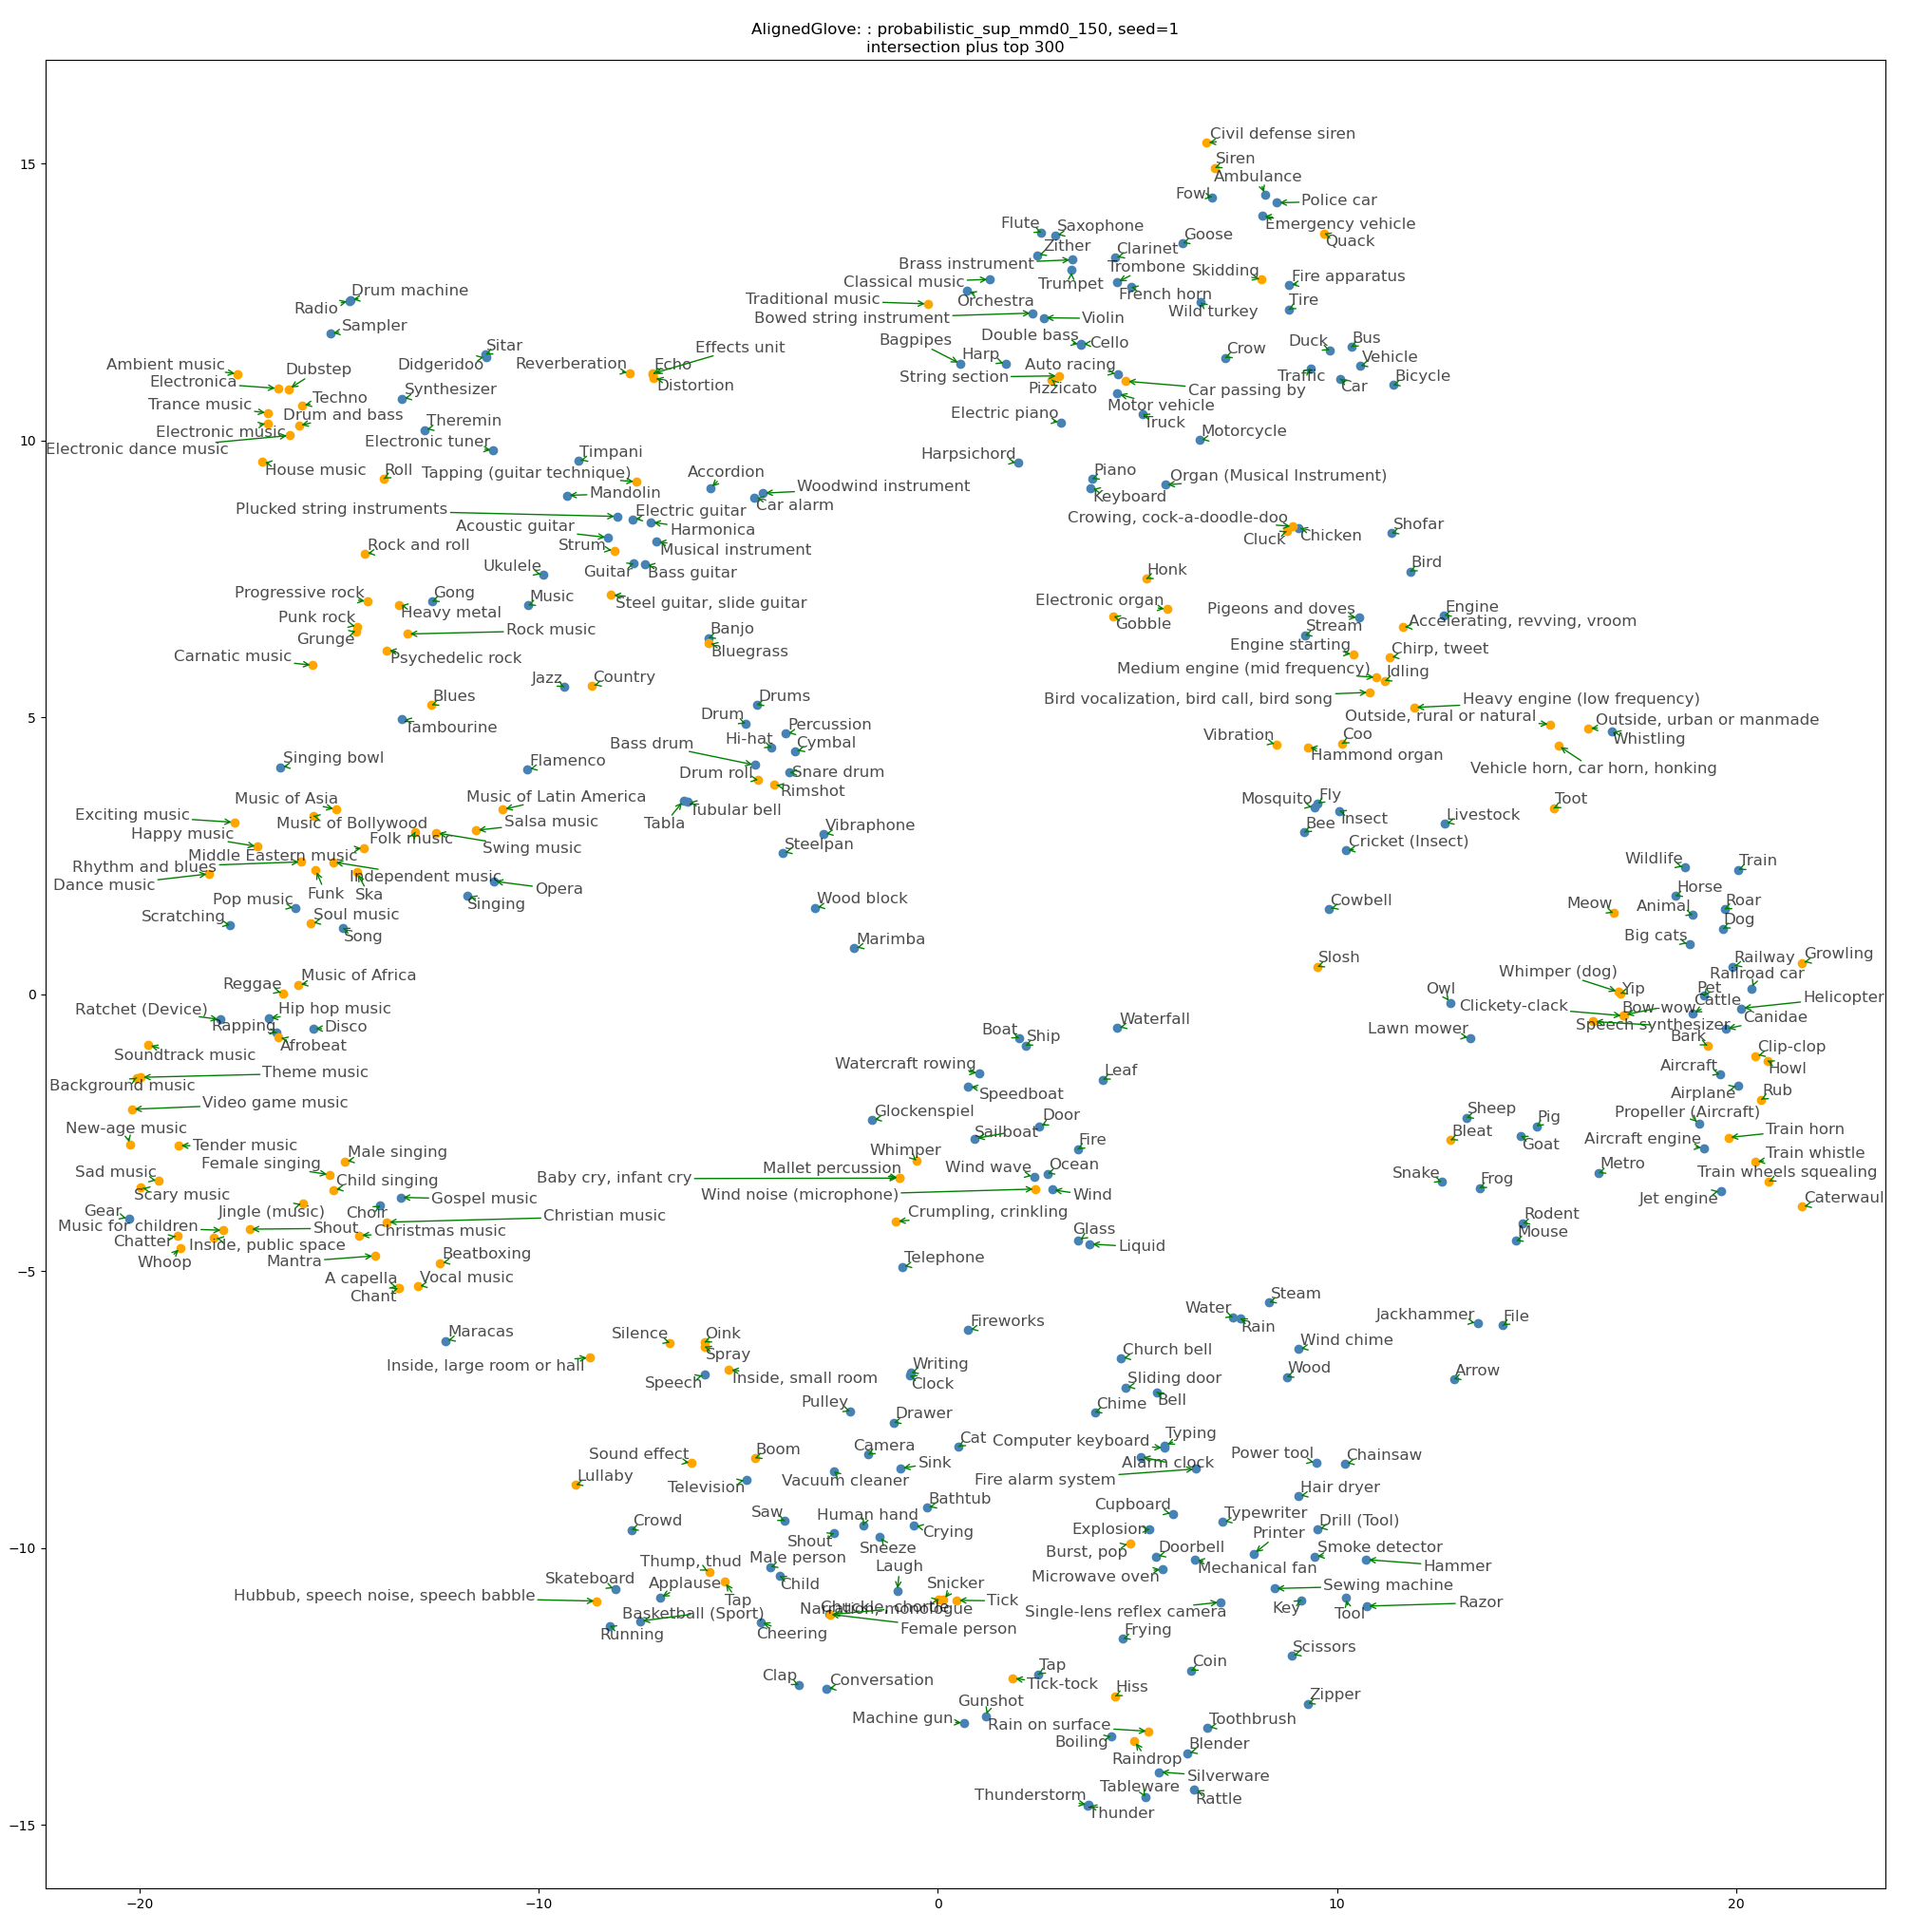
\includegraphics[width=\textwidth]{images/results/intersection_top300_tsne_audioset_probabilistic_sup_mmd0_150_AlignedGlove_1.png}
    \caption{
        \label{fig:audiosetaligned}
        t-SNE plot of concept embeddings for AudioSet that are in the intersection of both domains (blue points) or in the top 300 most frequent (orange points). These are the embeddings for alignment run without MMD. See Figure \ref{fig:audiosetzoom} for zoomed-in examples. 
    }
\end{figure}

In Figures \ref{fig:openimageszoom} and \ref{fig:audiosetzoom} below, we show some enlarged examples of clusters which show concepts in the intersection and out of the intersection. These clusters show that a good balance is struck between the GloVe loss and the distance loss / MMD; for an example of what happens when this balance is not found, see Figure \ref{fig:dysfunctional_clusters}, where the GloVe loss was not weighted sufficiently compared to the distance loss / MMD. 


\begin{figure}[H]

    \centering
    \fbox{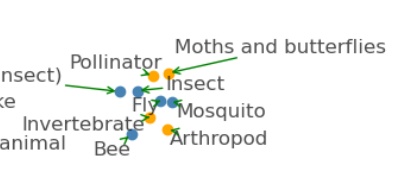
\includegraphics[width=0.4\textwidth]{images/results/openimages_zoom_insects.png}}
    \fbox{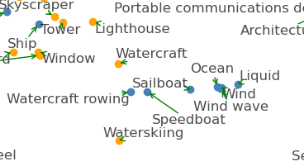
\includegraphics[width=0.4\textwidth]{images/results/openimages_zoom_ships.png}}
    \caption{\label{fig:openimageszoom}Enlarged view of two regions of the Open Images t-SNE plot, showing that concepts in and out of the intersection but semantically similar do form good clusters. As blue points denote concepts present in both domains and orange points denote concepts amongst the most frequent in the domain being examined, we want a mixture of orange and blue. }
\end{figure}

\begin{figure}[H]

    \centering
    \fbox{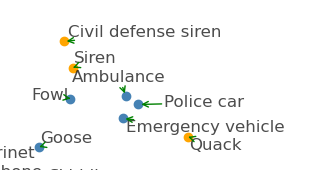
\includegraphics[width=0.4\textwidth]{images/results/audioset_zoom_sirens.png}}
    \fbox{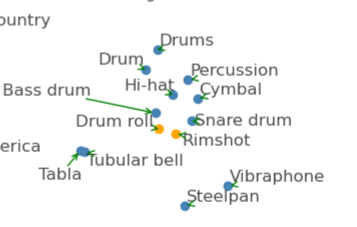
\includegraphics[width=0.4\textwidth]{images/results/audioset_zoom_drums.png}}
    \caption{\label{fig:audiosetzoom}Enlarged view of two regions of the AudioSet t-SNE plot showing the same phenomenon as described above.}
\end{figure}


\section{Statistics}

\subsection{Correlations}

We examine the correlations of self-similarity matrices over different random seeds, to get an idea of how consistent each set of embeddings is with itself. The similarity matrix of the embeddings for a given run is like a ``signature" of how the different concepts relate to each other within that run. We would like a high correlation of similarity matrices between runs, because that tells us that the algorithm is producing stable embeddings where concepts have the same degree of similarity with other concepts over many runs. 

\subsubsection{Average (Pearson) cross-correlation of self-similarity matrices of embedding means}

\begin{table}[H]
\centering
\begin{tabular}{lrrr}
\toprule
       &   Independent & Aligned     &  Aligned  \\
       &               & without MMD &  with MMD \\
\midrule
Open Images    & 0.590 $\pm$ 0.049 & 0.474 $\pm$ 0.044 &     0.420 $\pm$  0.040 \\
AudioSet    & 0.412 $\pm$ 0.045 &  0.399 $\pm$ 0.044  &      0.346  $\pm$ 0.043  \\
\bottomrule
\end{tabular}
\caption{\label{table:corrmeans}The similarity measure used for this table is the dot product of the means of the embeddings. The average is taken over all combinations of random seeds (1x2, 1x3, ..., 9x10).}
\end{table}

\subsubsection{Average (Pearson) cross-correlation of self-similarity matrices of samples of embeddings}
\begin{table}[H]
\centering
\begin{tabular}{lrrr}
\toprule
       &   Independent & Aligned     &  Aligned  \\
       &               & without MMD &  with MMD \\
\midrule
Open Images    & 0.589 $\pm$ 0.049 & 0.480 $\pm$ 0.040 &     0.434 $\pm$  0.040 \\
AudioSet    & 0.412 $\pm$ 0.044 &  0.399 $\pm$ 0.044  &      0.346  $\pm$ 0.043  \\
\bottomrule
\end{tabular}
\caption{\label{table:corrsamples}The similarity measure used for this table is mean of the dot product of 100 samples of each embedding (100 samples are taken, the pairwise dot product similarity computed, and the mean of those 100 similarity matrices is taken). This measure was used to take into account the variance of the embeddings, where the previous table used only the learned means of the embeddings. The average is taken over all combinations of random seeds (1x2, 1x3, ..., 9x10). It is not a typographical error that the values for AudioSet for mean of 100 similarity matrices are the same as the values for the embedding means in the previous table. }
\end{table}

The runs of the independently learned embeddings are more correlated with each other, compared to the equivalent calculation with the aligned embeddings. This means that the similarity matrices (of each run's embeddings with itself) are more consistent across runs. This correlation has dropped in the aligned runs, indicating that the output embeddings are less similar to themselves across runs. We can say that the alignment introduces more variation in the embeddings. MMD in particular seems to introduce more variability. 

\subsubsection{Mean Spearman correlation of entropy with frequency of occurrence}
\begin{table}[H]
\centering
\begin{tabular}{lrrr}
\toprule
       &   Independent & Aligned     &  Aligned  \\
       &               & without MMD &  with MMD \\
\midrule
Open Images    &  -0.179 $\pm$ 0.011 & 0.0421 $\pm$ 0.019 &     0.0362 $\pm$  0.012 \\
AudioSet    &  -0.400 $\pm$ 0.041 & -0.000539 $\pm$   0.074 &      0.0359  $\pm$ 0.026  \\
\bottomrule
\end{tabular}\\
\end{table}
There is a slight negative Spearman correlation between the entropy of a concept and its frequency of occurrence, in the independently learned cases. Entropies of less frequently occurring concepts are found to be higher, which is intuitively sensible; there is less information about those concepts so we would expect the variance, and therefore the entropy, to be higher. 

This correlation has largely disappeared in the aligned cases, being roughly around zero, indicating that there is now no relationship between the variance of the learned embedding for a concept and the frequency of that concept in the dataset. In this respect, the aligned probabilistic embeddings are less informative than the independent probabilistic ones. 
\subsection{Entropy plots of aligned embeddings}

\todo[inline]{I think the absolute positions of the entropy distributions for each run are not significant eg. comparing independent / aligned / aligned + MMD for seed = 1 is not relevant. I think it is the comparison of the distributions across all runs that is significant eg. independent for all seeds, aligned for all seeds, etc. }

\subsubsection{Open Images}

\begin{figure}[H]
\label{fig:entropyviolinimgs}
\centering
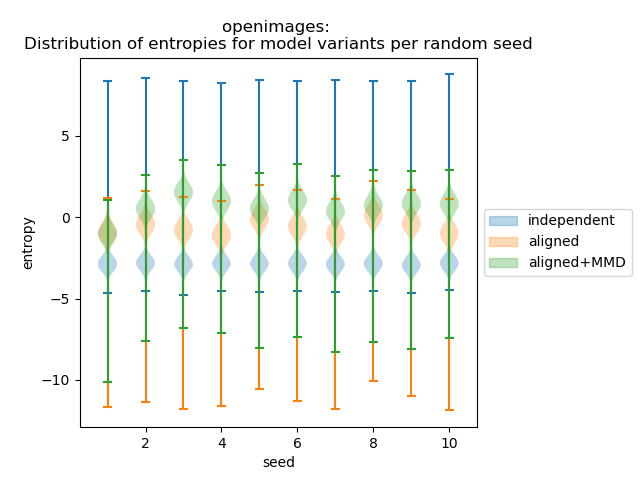
\includegraphics[width=\textwidth]{images/results/openimages_entropies_violin.png}
\caption{Violin plots of entropy distributions for independent embeddings, aligned without MMD and aligned with MMD. The entropy distribution for aligned embeddings is more variable between runs than that for independent embeddings. The use of MMD increases this variability. These results are consistent with the self-similarity correlations between runs shown in Tables \ref{table:corrmeans} and \ref{table:corrsamples}, which also indicated that the aligned embeddings were more unstable over different runs.}
\end{figure}

\subsubsection{AudioSet}

\todo[inline]{Does it mean anything that the aligned entropies are all lower in value (more negative) than aligned + MMD and independent? See above note on the relative comparisons per seed}

\begin{figure}[H]
\label{fig:entropyviolinaudio}
\centering
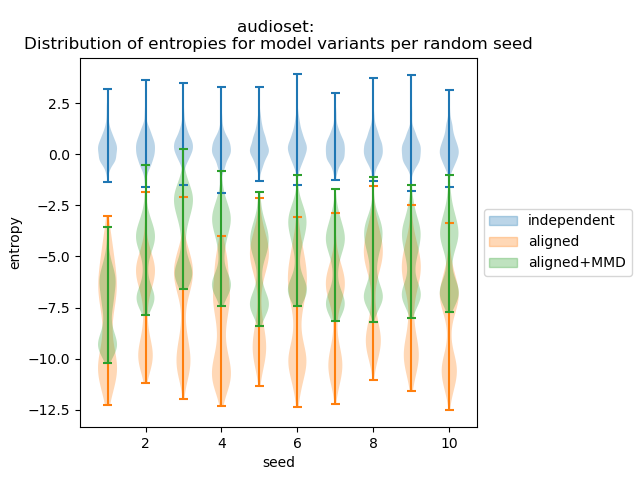
\includegraphics[width=\textwidth]{images/results/audioset_entropies_violin.png}
\caption{Violin plots of entropy distributions for independent embeddings, aligned without MMD and aligned with MMD. The aligned embeddings, whether run with or without MMD, show a bimodal entropy distribution and much greater variability than that of the independent embeddings.  These results are consistent with the self-similarity correlations between runs shown in Tables \ref{table:corrmeans} and \ref{table:corrsamples}, which also indicated that the aligned embeddings were more unstable over different runs. }
\end{figure}

\section{Alignment accuracy and embedding quality}

The table below shows the alignment accuracy for both domains, over 10 random seeds. Using the MMD statistic as a component of the loss marginally increased the accuracy. 

\begin{table}[H]
\centering
\begin{tabular}{lrrrr}
  \toprule
 \multicolumn{1}{c}{} & \multicolumn{2}{c}{Open Images} & \multicolumn{2}{c}{Audioset} \\
 \cmidrule(lr){2-3} \cmidrule(lr){4-5}
 %\multicolumn{5}{l}{Seed}
%       &    Open Images&               &  AudioSet    &            \\
{Seed} &    Without MMD &   With MMD   &  Without MMD &   With MMD \\
\midrule
1    &       0.9479 &        0.9478&    0.9478 &  0.9652  \\
2    &       0.9565 &        0.9826&    0.9696 &  0.9826  \\
3    &       0.9348 &        0.9565&    0.9565 &  0.9783  \\
4    &       0.9522 &        0.9652&    0.9565 &  0.9565  \\
5    &       0.9478 &        0.9609&    0.9435 &  0.9696  \\
6    &       0.9522 &        0.9739&    0.9739 &  0.9696  \\
7    &       0.9652 &        0.9652&    0.9478 &  0.9739  \\
8    &       0.9696 &        0.9522&    0.9609 &  0.9522  \\
9    &       0.9565 &        0.9565&    0.9609 &  0.9783  \\
10   &       0.9609 &        0.9522&    0.9652 &  0.9783  \\
\midrule                                                         
mean &       0.9543 &        0.9613 &   0.9583 &  0.9704  \\
\bottomrule
\end{tabular}
\end{table}

High alignment accuracy between embeddings in both domains does not necessarily mean the embeddings are good. Figure \ref{fig:dysfunctional_clusters} below is a t-SNE plot of aligned embeddings (reduced to 2 dimensions) of very high accuracy (97\%), meaning that the embeddings in Open Images and AudioSet are well aligned. However, the actual embeddings did not form good clusters; concepts that were related semantically tended not to be close in embedding space. 

\begin{figure}[H]

    \centering
    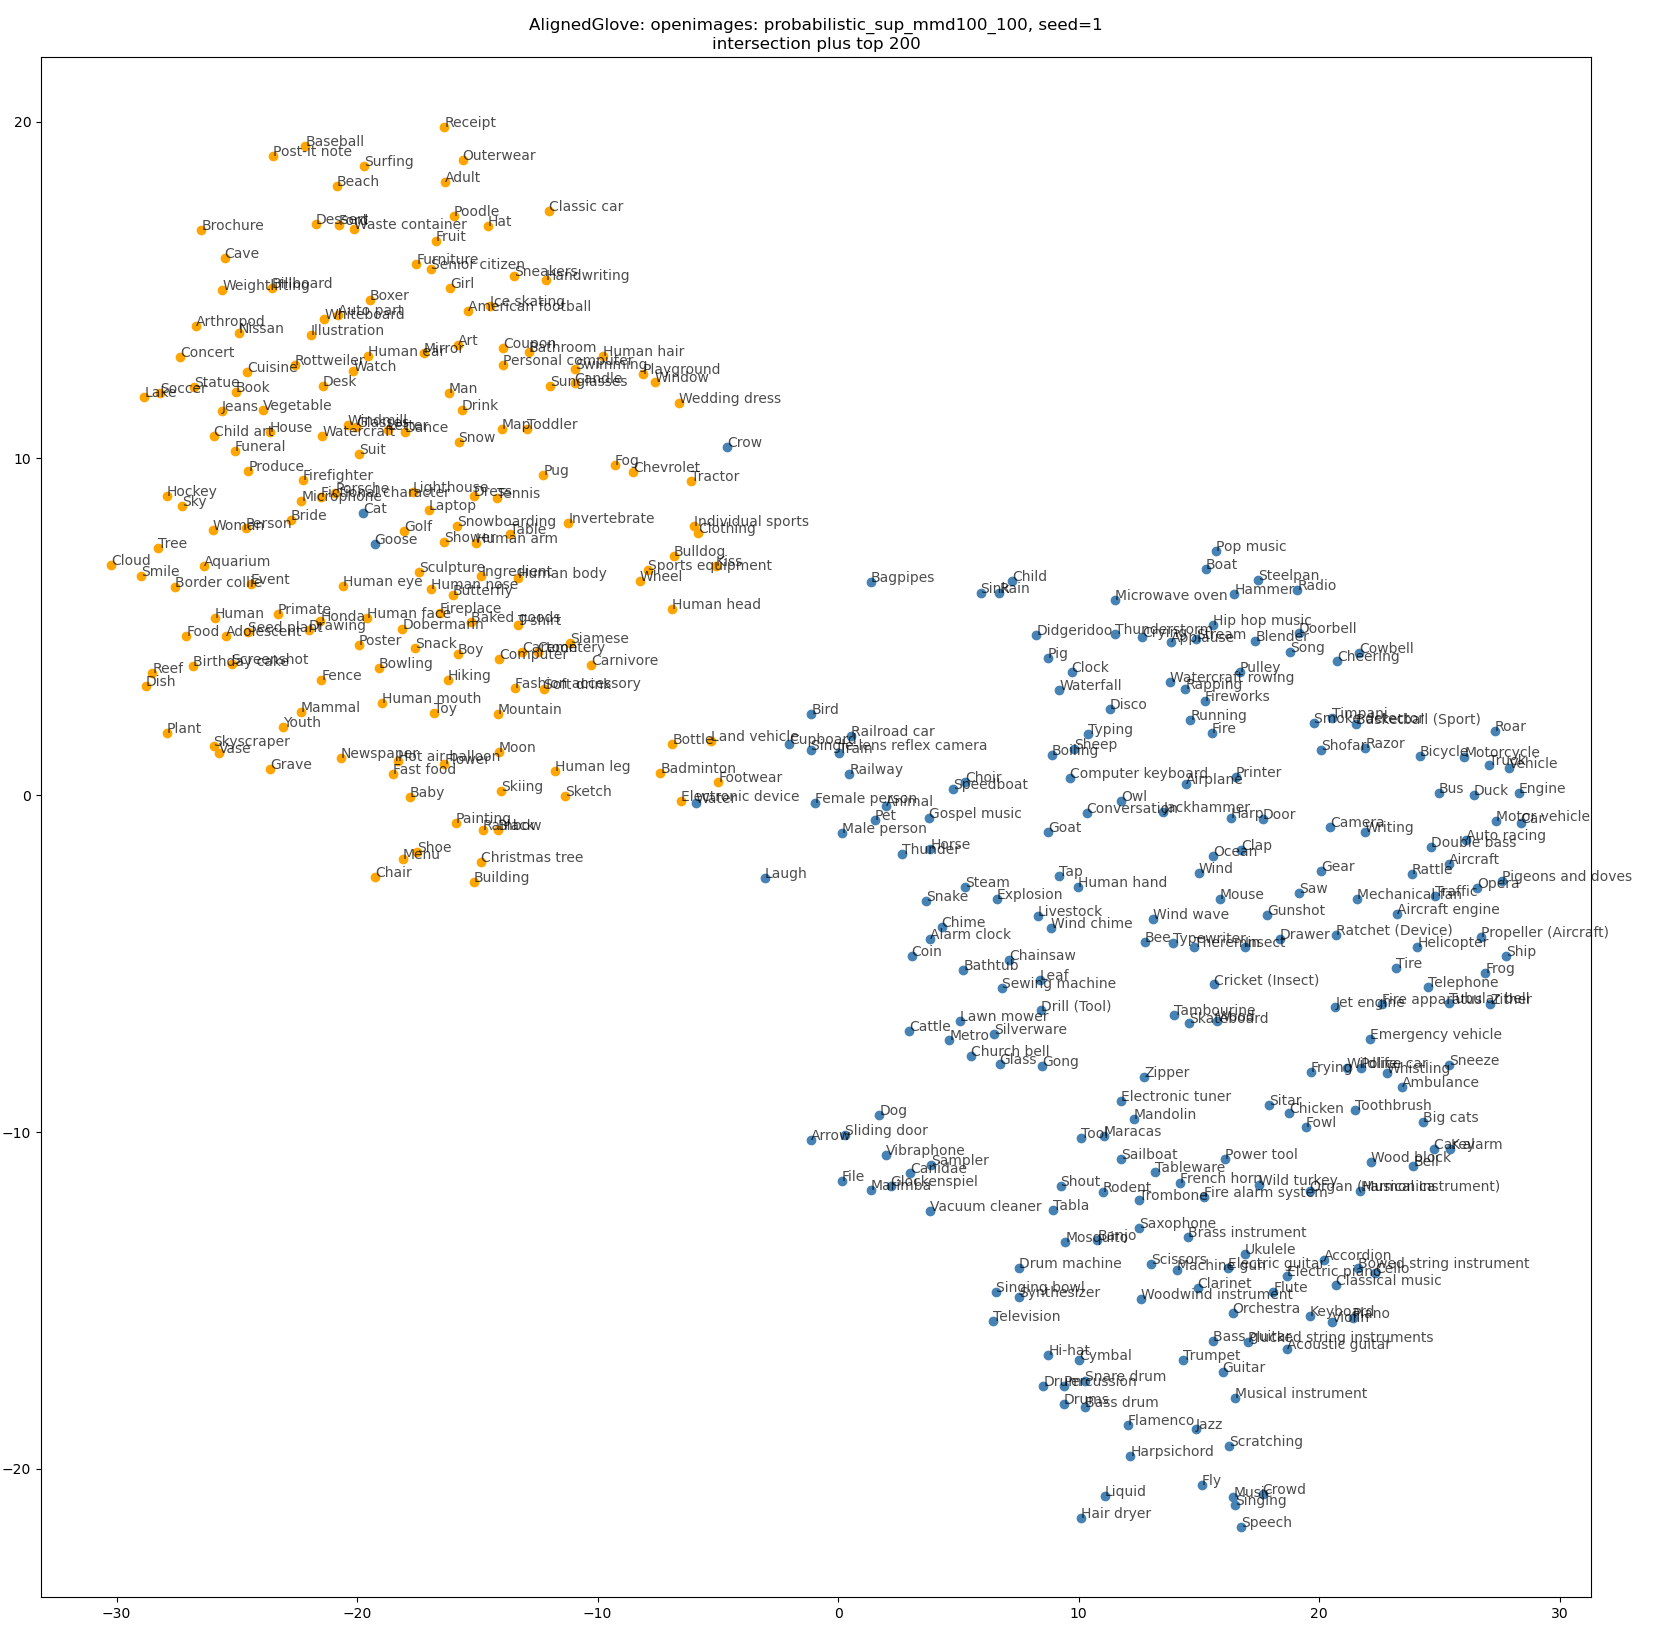
\includegraphics[width=1.0\textwidth]{images/method/probabilistic_aligned/dysfunctional_clusters.png}
    \caption{\label{fig:dysfunctional_clusters}
        The alignment accuracy for this set of embeddings is 97\%. The blue points denote concepts that are in the intersection of concepts (present in both Open Images and AudioSet). The orange points denote concepts that are in the 200 most frequent concepts occurring in Open Images. It is immediately visible that the algorithm has clustered concepts in the intersection degenerately; concepts that are in the intersection are more likely to be close to other concepts in the intersection rather than concepts that are semantically close.
    }
\end{figure}

Hence, alignment accuracy is insufficient as a metric. We can also examine the average Pearson correlations of the similarity matrices of the aligned and independent embeddings over 10 random seeds, for the two model variants: 

%inspect_results.py function aligned_vs_ind_corrs
\begin{table}[H]
\centering
\begin{tabular}{rrrr}
  \toprule
%       &    Open Images&               &  AudioSet    &            \\
\multicolumn{2}{c}{Open Images} & \multicolumn{2}{c}{Audioset} \\
\cmidrule(lr){1-2} \cmidrule(lr){3-4}
    Without MMD &   With MMD   &  Without MMD &   With MMD \\
\midrule
0.532 \pm 0.035 &   0.465 \pm 0.038 &   0.334 \pm 0.036 &  0.331 \pm 0.038  \\
\bottomrule
\end{tabular}
\end{table}

The above are aggregate statistics that only tell us that there is a positive correlation between the similarities of the aligned and independent embeddings. We do not know if the aligned embeddings are actually semantically more meaningful than the independent, or the other way around. 

\subsection{Comparing aligned embeddings with human similarity scores}

A plausible measure of embedding quality would be a comparison of the similarity of concept pairs as calculated from embeddings, with the similarity of concept pairs as evaluated by humans. In order to do this, we need to find datasets that capture human ratings of similarity. If our alignment algorithm is good, we should expect that the aligned embeddings are of higher quality than the independently learned embeddings and correlate more highly with human similarity judgement. 

\textbf{MTURK-771}: The MTURK-771 dataset was created by the authors of \cite{mturk771}, a study in learning the relatedness of word pairs. The predictions are tested by comparing the Spearman correlation of its predictions with human judgements. The MTURK-771 dataset comprises 771 pairs of words with human-rated similarity scores, collected using the Amazon Mechanical Turk tool. The intersection of the 771 word pairs with our Open Images and AudioSet concepts was small - 171 (0.013\%)  for Open Images and only 3 (0.0071\%) for AudioSet. 

\textbf{WordNet}: The WordNet \cite{WordNet} lexical database contains English nouns, verbs and adjectives grouped according to synonymy (semantic similarity) and hypernymy/hyponymy (hierarchy). Words are represented by ``synsets" which denote a particular sense of the word (for example, ``orange" may refer to the colour or the fruit). Therefore, one word may map to several synsets. The relationships between word senses were hand-encoded from various corpora and thesauri, which themselves were human-curated; therefore, we consider the lexical and semantic information contained within WordNet to be an appropriate representation of human judgement. The WordNet database can be accessed directly from the \texttt{nltk} Python package. 

There is a substantial overlap between pairs of words found in WordNet and pairs of concepts from our dataset.  Out of approximately 128 million (128005400) nonzero pairs occurring in Open Images, approximately 27 million (27052350, 21.1\%) are also present in WordNet. Out of 42002 nonzero pairs in AudioSet, 19208 (45.7\%) are also present in WordNet. 

\textbf{ILSVRC}: A third available dataset originates from a prototype model for \cite{RoadsLoveCVPR}, in which human similarity judgements of pairs of concepts were collected to supplement the ImageNet Large-Scale Visual Recognition Challenge (ILSVRC) 2012 task. This dataset will be referred to as the ``enhanced ILSVRC" dataset. These judgements were collected from participants using Amazon Mechanical Turk. The data collection process used probabilistic techniques for trial selection to maximise the expected information gain from each trial. In this dataset, 147070 (0.115\%) pairs overlap with Open Images, and 93 (0.221\%) pairs overlap with AudioSet. One word, ``tick", was removed from the AudioSet pairs when computing the comparison, because that label as used in AudioSet is used to describe the sound and not the insect. We know that the ImageNet label corresponds to the insect. 

We adopt the method used by \cite{mturk771} of comparing the Spearman correlation of the similarity of our embedding concept pairs with the similarity of the human-measured dataset to evaluate the quality of aligned embeddings compared to independently learned embeddings. The Spearman correlation is used because we wish to evaluate whether there is a monotonic relationship, and the similarity measures all use different scales. The cosine similarity measure is used as it contains the dot product, which is an input into the GloVe algorithm that generates the embeddings, and the magnitude of the embeddings is not meaningful. 

The similarity of two concepts with indexes $i$ and $j$ in embedding space is:

\begin{equation*}
s_{ij} = \frac{\vece_i \cdot \vece_j}{||\vece_i||_2 \medspace ||\vece_j||_2}
\end{equation*}

where $\vece_i$ represents the $i$-th embedding.

If the correlation with the human similarity dataset is higher for aligned embeddings than for independently learned embeddings, this indicates that the alignment process is adding value, resulting in more cognitively plausible embeddings. This is because it indicates that the aligned embedding pairs are in aggregate more like human judgement of similarity than the independent embedding pairs. We will use this as a metric for embedding quality, where higher quality means more similar to human judgement.  We evaluate the model variants with and without MMD by this metric to assess the effect of MMD. 

The MTURK-771 and enhanced ILSVRC datasets are pre-existing mappings of concept pairs to similarity values, which can be used without any preprocessing. There is no such WordNet dataset of direct similarity, so we have to construct one. WordNet makes available similarity measures between synsets that can be computed directly from the Python library. We choose the Leacock-Chodorow (LCH) similarity measure \cite{LeacockChodorow}, which takes the shortest path between the two synsets, scaled by the maximum depth from the top of the taxonomy tree of the two synsets (this measure was chosen as it is the only one that combines path length between nodes and depth of the tree).  

As a single word or phrase may map to several synsets, and we have no sense information in our Open Images / AudioSet concept names to disambiguate between choices, we may have more than one feasible synset pair per concept pair in our dataset. We use the following heuristic algorithm to decide which specific synset pair's scores to use:

\begin{itemize}
    \item Check every pair in the domain (Open Images or AudioSet) that appears at least once (its entry in the co-occurrence matrix is nonzero).
    \item Convert the pair words to lowercase with spaces replaced with underscores (this is the WordNet naming scheme).
    \item Check if both words have synsets in WordNet. If either does not, ignore the pair.
    \item For each combination of the first 2 synsets for each word (up to 4 pairs in total), compute the LCH similarity if both elements in the pair have the same part of speech, otherwise ignore the pair. \footnote{WordNet similarity is not defined for synsets which do not have the same parts of speech. } This is to handle pairs like ``mandarin orange" and ``orange". ``Mandarin orange" has two synsets; the first refers to the mandarin orange tree, and the second refers to the fruit. Therefore the second ``mandarin orange" synset matches the first ``orange" synset (which denotes the fruit, rather than the colour) more closely. One mode of failure for this algorithm is for words that occur in both Open Images and AudioSet but with different meanings, for example, ``tap" and ``tick" are different concepts when referring to objects or sounds. 
    \item The WordNet similarity for the pair is taken to be the largest such value. This algorithm will therefore be biased high.
\end{itemize}


\subsection{Results of comparison with human similarity metrics}

\subsubsection{Degree of overlap of human similarity datasets with domain pairs}

These are the percentages of data overlap for the different domains:

\begin{table}[H]
\centering
\begin{tabular}{lrr}
\toprule
{Human similarity dataset} &  Open Images &   AudioSet\\
\midrule
MTURK-771    &     0.013\% &  0.0071\%  \\
WordNet    &     21.1\% &  45.7\%  \\
enhanced ILSVRC    &    0.115\% &  0.221\% \\
\bottomrule
\end{tabular}
\end{table}

\subsubsection{Open Images, Spearman correlation with human similarity metrics}
\begin{table}[H]
\centering
\begin{tabular}{lrrrrrrrrr}
  \toprule

%   &     &   MTURK-771        &               &      &    WordNet       &               &     &  ILSVRC           & \\
\multicolumn{1}{r}{} & \multicolumn{3}{c}{MTURK-771} & \multicolumn{3}{c}{WordNet} & \multicolumn{3}{c}{ILSVRC} \\
\cmidrule(lr){2-4} \cmidrule(lr){5-7} \cmidrule(lr){8-10}
{Seed} &  Ind. &   Aligned &  Aligned  & Ind. &   Aligned &  Aligned  & Ind. &   Aligned &  Aligned   \\
{}     &              &           & +MMD      &            &            & +MMD      &             &           &   +MMD \\
\midrule
1    &     0.357 &  0.306 &   0.331 &     0.205 &  0.229 &    0.228 &   0.524 &  0.493 &  0.488  \\
2    &     0.343 &  0.271 &   0.296 &     0.196 &  0.221 &    0.230 &   0.471 &  0.460 &  0.458  \\
3    &     0.376 &  0.338 &   0.287 &     0.200 &  0.240 &    0.240 &   0.483 &  0.486 &  0.433  \\
4    &     0.343 &  0.300 &   0.290 &     0.210 &  0.233 &    0.229 &   0.514 &  0.531 &  0.482 \\
5    &     0.358 &  0.256 &   0.225 &     0.191 &  0.226 &    0.226 &   0.505 &  0.466 &  0.456  \\
6    &     0.374 &  0.309 &   0.271 &     0.207 &  0.239 &    0.237 &   0.541 &  0.473 &  0.451  \\
7    &     0.347 &  0.297 &   0.292 &     0.208 &  0.229 &    0.239 &   0.506 &  0.468 &  0.447  \\
8    &     0.343 &  0.284 &   0.283 &     0.215 &  0.217 &    0.218 &   0.553 &  0.458 &  0.468  \\
9    &     0.340 &  0.279 &   0.271 &     0.217 &  0.224 &    0.233 &   0.508 &  0.463 &  0.439  \\
10   &     0.367 &  0.267 &   0.284 &     0.207 &  0.225 &    0.230 &   0.531 &  0.464 &  0.452  \\
\midrule                                                                                         
mean &     0.355 &  0.291 &   0.283 &     0.205 &  0.228 &    0.231 &   0.514 &  0.476 &  0.458  \\
\bottomrule
\end{tabular}
\end{table}

\subsubsection{Open Images, differences of Spearman correlation between aligned model variant and independently learned embeddings}


\begin{table}[H]
\centering
\begin{tabular}{lrrrrrr}
  \toprule
  
%       &   MTURK-771 &           &  WordNet  &           &  ILSVRC  &            \\
\multicolumn{1}{r}{} & \multicolumn{2}{c}{MTURK-771} & \multicolumn{2}{c}{WordNet} & \multicolumn{2}{c}{ILSVRC} \\
\cmidrule(lr){2-3} \cmidrule(lr){4-5} \cmidrule(lr){6-7}
{Seed} &   Aligned   &  Aligned  &   Aligned &  Aligned  &  Aligned &  Aligned   \\
{}     &             & +MMD      &            & +MMD     &          &   +MMD     \\
\midrule
1    &     -0.0512 &    -0.0260  &   0.0244 &     0.0234 &    -0.0305 &    -0.0353   \\
2    &     -0.0716 &    -0.0465  &   0.0255 &     0.0346 &    -0.0107 &    -0.0130   \\
3    &     -0.0374 &    -0.0884  &   0.0402 &     0.0402 &     0.00349 &    -0.0495   \\
4    &     -0.0433 &    -0.0530  &   0.0232 &     0.0185 &     0.0174 &    -0.0322   \\
5    &     -0.102  &    -0.133   &   0.0354 &     0.0356 &    -0.0385 &    -0.0484   \\
6    &     -0.0650 &    -0.103   &   0.0320 &     0.0301 &    -0.0686 &    -0.0904   \\
7    &     -0.0509 &    -0.0552  &   0.0216 &     0.0308 &    -0.0383 &    -0.0595   \\
8    &     -0.0592 &    -0.0599  &   0.00189 &    0.00313 &   -0.0948 &    -0.0851   \\
9    &     -0.0614 &    -0.0686  &   0.00696 &    0.0166 &    -0.0448 &    -0.0691   \\
10   &     -0.0995 &    -0.0828  &   0.0184 &     0.0235 &    -0.0674 &    -0.0793   \\
\midrule                                                                                          
mean &     -0.0641 &    -0.0716  &   0.0230 &     0.0256 &    -0.0373 &    -0.0562   \\
\bottomrule
\end{tabular}
\end{table}


For Open Images, using the WordNet comparison metric, the aligned embeddings are more correlated with human similarity than the independently learned embeddings, as the mean Spearman correlation of alignment pairwise cosine similarity with WordNet similarity is greater for aligned embeddings than for independent embeddings. 

The reverse is observed with the MTURK-771 comparison metric, but we do note that this is a very small dataset of only 170 pairs present in both Open Images (out of 120 million pairs) and MTURK-771. The same phenomenon as with MTURK-771 is also observed when comparing with the ILSVRC metric, where the aligned embeddings are less correlated with human judgement than the independently learned embeddings degree of correlation with human judgement. 

However, the ILSVRC dataset is unbalanced, and some of the choices of included concepts are strange. There are 1000 concepts present in it, of which 124 are different breeds of dog. In fact, 398 of the concepts present in the ILSVRC are different types of animal. There are some concepts in the selected 1000 that almost certainly are not amongst the most common humanly known concepts, for example, ``shoji"\footnote{A Japanese sliding door made of paper.} and ``bicycle-built-for-two" (with ``bicycle" not present). The only flowers present are ``cardoon" \footnote{A type of thistle.}, ``daisy" and ``yellow lady's slipper". In short, the concepts represented in the ILSVRC dataset do not appear to be a very good sample of human concepts. To investigate whether the imbalance of the dataset was affecting results, runs were tried of the ILSVRC dataset excluding all the animals and then only including animals, but the results were broadly the same. 

\textbf{Given that the overlap of WordNet pairs with our domain pairs is considerable (21.1\% for Open Images and 45.7\% for AudioSet), we think that the higher correlation with WordNet similarity for aligned Open Images embeddings constitutes evidence that embedding quality is improved by alignment.} This would be consistent with hypotheses that multi-task learning adds value by producing a model that generalises better.

However, playing devil's advocate, we do also point out that the WordNet similarity score is an artificial score inferred from properties of the WordNet database, whereas the MTURK-771 and  ILSVRC similarity measures are directly collected from humans. 

Using the MMD as a component of the loss appears to increase accuracy, as well as alignment quality as measured against the WordNet metric. If comparing to the MTURK-771 and ILSVRC datasets, using MMD appears to decrease the alignment quality.  

\subsubsection{AudioSet, Spearman correlation with human similarity metrics}

MTURK-771 is excluded from this comparison, as with only 3 pairs present in both MTURK-771 and AudioSet, no meaningful results could be obtained. 

\begin{table}[H]
\centering
\begin{tabular}{lrrrrrr}
  \toprule
%       &       &   WordNet &           &      &  ILSVRC   &            \\
\multicolumn{1}{r}{} & \multicolumn{3}{c}{WordNet} & \multicolumn{3}{c}{ILSVRC} \\
\cmidrule(lr){2-4} \cmidrule(lr){5-7} 
{Seed} &  Ind. &   Aligned &  Aligned  & Ind. &   Aligned &  Aligned   \\
{}     &       &           & +MMD      &      &           &   +MMD     \\
\midrule
1    &    0.139 &  0.163 &   0.153 &   0.635 &  0.683 &   0.502    \\
2    &    0.132 &  0.130 &   0.147 &   0.585 &  0.687 &   0.651   \\
3    &    0.157 &  0.175 &   0.133 &   0.647 &  0.428 &   0.617   \\
4    &    0.147 &  0.148 &   0.169 &   0.560 &  0.610 &   0.649   \\
5    &    0.116 &  0.151 &   0.152 &   0.562 &  0.513 &   0.578   \\
6    &    0.144 &  0.134 &   0.125 &   0.631 &  0.609 &   0.504   \\
7    &    0.150 &  0.134 &   0.170 &   0.539 &  0.563 &   0.546   \\
8    &    0.140 &  0.183 &   0.128 &   0.553 &  0.675 &   0.682   \\
9    &    0.147 &  0.136 &   0.187 &   0.524 &  0.718 &   0.681   \\
10   &    0.150 &  0.166 &   0.143 &   0.607 &  0.717 &   0.699   \\
\midrule                                                                   
mean &    0.142 &  0.152 &   0.151 &   0.584 &  0.620 &   0.611   \\
\bottomrule
\end{tabular}
\end{table}



\subsubsection{AudioSet, differences of Spearman correlation between aligned model variant and independently learned embeddings}


\begin{table}[H]
\centering
\begin{tabular}{lrrrr}
\toprule
%       &     WordNet  &           &  ILSVRC  &            \\
\multicolumn{1}{r}{} & \multicolumn{2}{c}{WordNet} & \multicolumn{2}{c}{ILSVRC} \\
\cmidrule(lr){2-3} \cmidrule(lr){4-5}
{Seed} &      Aligned &  Aligned  &  Aligned &  Aligned   \\
{}     &               & +MMD     &          &   +MMD     \\
\midrule
1    &    0.0237 &     0.0138  &   0.0489 &    -0.132    \\
2    &   -0.00278 &     0.0144 &   0.102  &     0.0662   \\
3    &    0.0176 &    -0.0237  &  -0.219  &    -0.0293   \\
4    &    0.00162 &     0.0221 &   0.0497 &     0.0886   \\
5    &    0.0350 &     0.0361  &  -0.0488 &     0.0160   \\
6    &   -0.00988 &    -0.0189 &  -0.0218 &    -0.127    \\
7    &   -0.0156 &     0.0202  &   0.0237 &     0.00677  \\
8    &    0.0423 &    -0.0127  &   0.122  &     0.129    \\
9    &   -0.0117 &     0.0401  &   0.194  &     0.157    \\
10   &    0.0160 &    -0.00696 &   0.110  &     0.0918   \\
\midrule                                                                    
mean &    0.00964 &     0.00844 &   0.0361 &     0.0267  \\
\bottomrule
\end{tabular}
\end{table}

\textbf{When compared with both WordNet and ILSVRC, AudioSet aligned embeddings are more correlated with human similarity judgement than the independently learned embeddings.}  However, only 93 pairs present in AudioSet overlap with ILSVRC pairs, so this is not a large sample for comparison. It is also subject to the vagaries of the ILSVRC dataset concept choice, as discussed in the previous section. We observe an asymmetry, where Open Images improves AudioSet with respect to ILSVRC, but AudioSet does not improve Open Images, which could be due to the fact that there are nearly 40 times as many concepts in Open Images than AudioSet, so there is simply much more information there to assist with alignment of AudioSet than there is in the other direction. 

Similar to Open Images, including MMD in the loss function increases accuracy, but it slightly decreases alignment quality when compared to independently learned embeddings using both WordNet and ILSVRC metrics.

\subsection{Overall results}
\textbf{When compared with WordNet similarity, both domains' aligned embeddings showed more correlation with human similarity judgement than the equivalent independently learned embeddings. This is some evidence to show that the information gained from learning both domains simultaneously results in both domains' embeddings being of higher quality.} 
 
This is consistent with our hypothesis that constraining the embedding learning problem for both domains by adding alignment would allow each domain to act as an inductive bias for the other, leading to a better global solution. This also matches the multi-task learning research showing that learning from multiple sources results in models that generalise better.


\subsection{Embedding stability}

Another metric of embedding quality is their stability over multiple runs. As previously mentioned, the stochasticity in the GloVe embedding training means that different embeddings are produced for different runs, corresponding to different local minima. The structures of these are not the same from run to run, as we saw in a table of the top 5 nearest neighbours for various concepts, over different random seeds (Tables \ref{table:cat}, \ref{table:subclasscat}). 

We use two measures of stability; one is the metric mentioned in \cite{WordEmbeddingStability}, a simple count of the number of intersecting concepts in the 5 nearest neighbours of any concept, over 10 seeds (divided by 5 to normalise to 1). We also define an alternate similarity metric which is easier to plot and visualise as follows:

\begin{itemize}
    \item Measure the size of the union of all the top 5 nearest neighbours of a concept, by Euclidean distance, for 10 random seeds. Let this be $C$. 
    \item Take the mean of $5/C$ for the top 300 concepts in Open Images and Audioset.
    \item If the embeddings were very stable, then the top 5 nearest neighbours of a concept over all runs should be the same, and the stability will be 1. If they are very unstable, the top 5 nearest neighbours will be different with each run, and the stability will be a small number. 
\end{itemize}

\subsubsection{Mean stability of embeddings by model variant}

Empirically, alignment appears to decrease stability of the embeddings, meaning that the nearest neighbours of a particular concept (measured by Euclidean distance) tend to change more over different random seeds. Intuitively this is reasonable. Training aligned probabilistic embeddings involves more variables and a more complex loss function, so we might expect the variances to be greater. 

\begin{table}[H]
\centering
% generated by inspect_results.py: print(sdf.to_latex())
\begin{tabular}{lllrr}
\toprule
Embedding type  & MMD    & Domain          & Union metric & Intersection metric         \\
\midrule
Aligned & Without MMD   & Open Images &  0.2373 & 0.0733\\
            &     & AudioSet &  0.2108 & 0.0535\\
\cmidrule(lr){2-5}
            & With MMD & Open Images &  0.2103 & 0.0527\\
                   &     & AudioSet &  0.2248 & 0.0816\\
\cmidrule(lr){1-5}
Independent & N/A   & Open Images &  0.2900 & 0.1013 \\
                   &     & AudioSet &  0.3901 & 0.3311 \\
\bottomrule
\end{tabular}\\
\end{table}

\subsubsection{Plots of stability by relative frequency}

The per-item plots very clearly show that alignment decreases the stability of the embeddings, as seen from the distribution of the stability values per rank of concept frequency. For the independently learned embeddings, some concepts have a stability of 1.0 which means that over 10 random seeds, the 5 nearest neighbours of those concepts did not change over all runs. The aligned embeddings do not have any concepts with a stability of 1.0. 

\cite{WordEmbeddingStability} ran stability analysis for word embeddings across languages. They found that languages with higher morphological complexity tended to be less stable than languages with less complex morphology. The morphological complexity of a language depends on the relationships between the words in that language; more complex relationships means a higher morphological complexity \cite{MorphologicalComplexity}. If we draw a parallel between the combined (AudioSet + Open Images) embeddings and language, it can be suggested that the combined embeddings have more complex relationships, so we would expect them to be less stable. 

\begin{figure}[H]
    \centering
    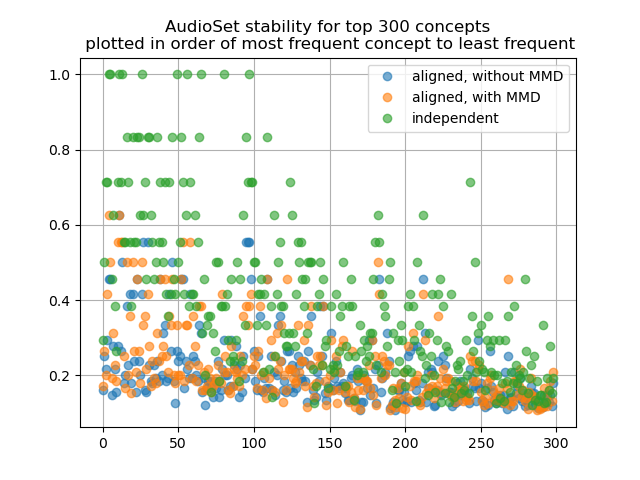
\includegraphics[width=0.45\textwidth]{images/results/audioset_stability.png}
    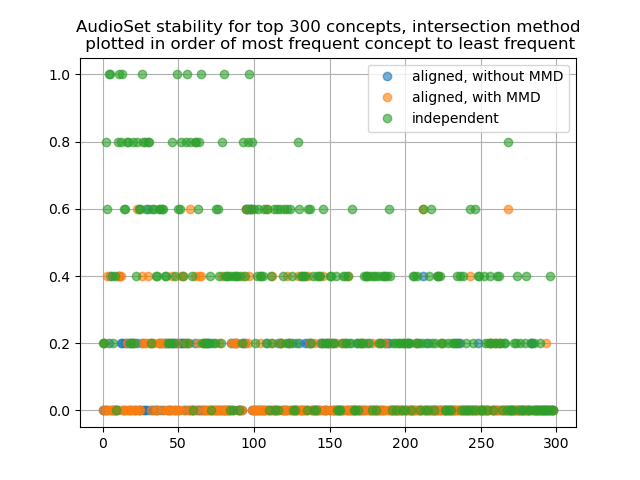
\includegraphics[width=0.45\textwidth]{images/results/audioset_stability_ixn.png}
    \caption{
        Stability of model variants for AudioSet. y-axis is relative frequency of concepts (most frequent = 0)
    }
\end{figure}


\begin{figure}[H]
    \centering
    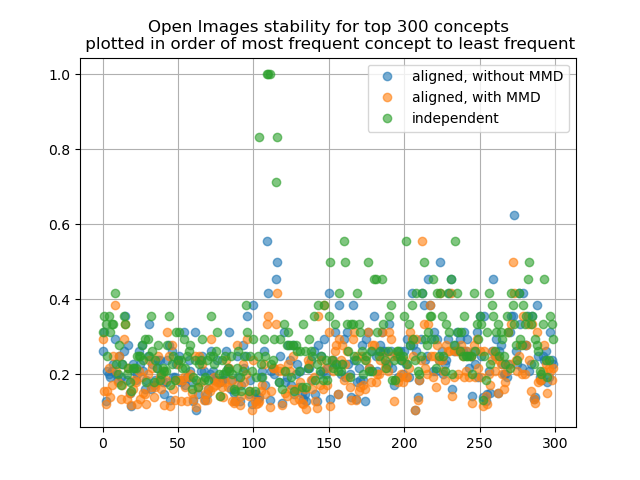
\includegraphics[width=0.45\textwidth]{images/results/openimages_stability.png}
    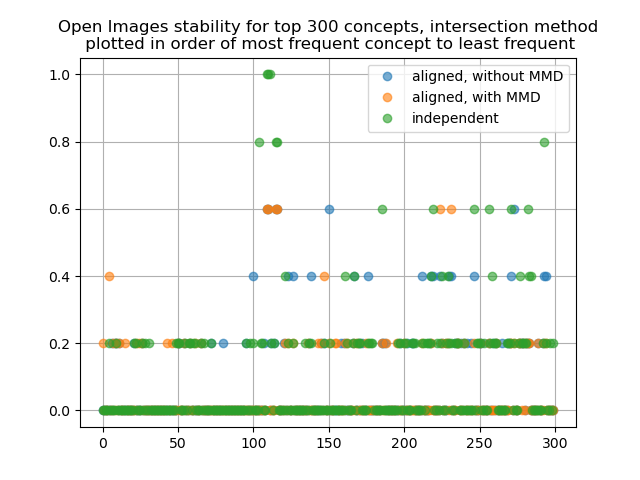
\includegraphics[width=0.45\textwidth]{images/results/openimages_stability_ixn.png}
    \caption{
        Stability of model variants for Open Images. y-axis is relative frequency of concepts (most frequent = 0)
    }
\end{figure}

\subsection{Other findings}
\subsubsection{The role of MMD}

Using MMD as a loss function has the effect of forcing $f(x)$ and $y$ to have the same distribution, and  $g(y)$ and $x$ to have the same distribution. Therefore it is reasonable that it should have a positive effect on alignment accuracy. However if the weighting of the MMD loss is high relative to glove loss, there is more pressure for distribution  matching but less pressure for good embeddings which can result in dysfunctional embeddings where all the concepts in the intersection are clustered together as shown in Figure \ref{fig:dysfunctional_clusters}. 

\subsubsection{Entropies and variances}

The entropies no longer correlate negatively with frequency of concepts, in the aligned embeddings. It is more appropriate to say they are now close to independent of the frequency of concepts, since the correlation is near zero. 

\subsubsection{GloVe loss scaling}
If the GloVe loss was not scaled by the ratio of concepts (see Section \ref{section:gloveloss}), the effect of this was to cause the (intersecting) concepts in the embedding to exhibit poor semantic organization.



%\begin{itemize}
%    \item Alignment accuracies of greater than 95\% were achieved for both domains ($f(x) \rightarrow y$ and $g(y) \rightarrow x$). % This was contingent on taking 10 samples for each embedding in each batch. If only 1 sample per embedding was taken, only 90\% accuracy was achieved. This is probably because using 10 samples acts like data augmentation. 
%\end{itemize}